\documentclass[11pt,letterpaper,notitlepage]{article}

\usepackage{fullpage}
\usepackage{enumerate}
\usepackage{amsmath}
\usepackage{amsthm}
\usepackage{paralist}
\usepackage{hyperref}
\usepackage{cite}
\usepackage{clrscode3e}
\usepackage{appendix}
\usepackage{framed}
\usepackage{graphicx}

\hypersetup{
    colorlinks,%
    citecolor=black,%
    filecolor=black,%
    linkcolor=black,%
    urlcolor=black
}

\title{An Analysis of the SPDY Protocol as a Candidate for HTTP/2.0}
\date{\today}
\author{Brian Stack\thanks{ bis12@case.edu, Case Western Reserve University,
Cleveland, OH 44106}, Tom Dooner\thanks{ ted27@case.edu }}


\begin{document}
\maketitle
\setcounter{tocdepth}{1}
\tableofcontents
\begin{abstract}
The HTTP/1.1 specification is now well over a decade old~\cite{rfc2616}. Updates
have been constantly made to the specification, in an attempt to clear up
discrepancies or clarify murky parts of the document.  The most recent attempt
at this was made as recently as April of 2012~\cite{rfc6585}.  Even so, as the web grows
and changes, the venerable spec is beginning to show its age.  Companies such as
Google and Facebook who serve massive portions of the daily web traffic are
pushing the limit of HTTP performance, mostly due to the outdated design
assumptions made during the original specification of the protocol.  In March of
2012, httpbis (the IETF's HTTP working group) updated their charter to
include a directive of creating a new specification -- HTTP/2.0.  One of the
most likely starting points for the new protocol will be Google's
SPDY~\cite{spdyspec}.  This paper will inspect this protocol to analyze its
performance and weigh it against the design compromises it makes in order to
help decide whether or not this is a good direction for the HTTP specification
to go.
\end{abstract}

%%%%%%%%%%%%%%%%%%%%%%%%%%%%%%%%%%%%%%%%%%%%%%%%%%%%%%%%%%%%%%%%%%%%%%%%%%%%%%%
\section{Background}
\label{sec:background}
%%%%%%%%%%%%%%%%%%%%%%%%%%%%%%%%%%%%%%%%%%%%%%%%%%%%%%%%%%%%%%%%%%%%%%%%%%%%%%%
HTTP is one of the most widely used application-level protocols. Initially
written in 1996~\cite{http1rfc}, HTTP was written for a different era of web
sites -- before streaming video websites, before asset-heavy web pages, and
before mostly-Javascript web applications like Google's Gmail, Twitter, and
Facebook.

Although HTTP was amended in 1999 to include better support for caching, the
ability to reuse connections, and other helpful features, the World Wide Web
landscape has changed significantly since then -- led by big technology
companies desiring to optimize application speed and user experience.

The IETF's httpbis working group is responsible for maintaining and developing
the HTTP specification, including all aspects pertaining to developing a new
HTTP specification, HTTP/2.0. The most recent httpbis working group charter
mentions the following goals for HTTP/2.0~\cite{httpbis-charter}:
\begin{itemize}
\item Significantly improve performance in common use cases
\item Make more efficient use of network resources
\item Must be deployable on the current internet
\item Maintain ease of deployment
\item Updated security to modern standards
\end{itemize}

The most important part of the goals that is not explicitly mentioned is that
these proposals must maintain semantic equivalence with the currently
implemented HTTP specification; changes may only be made to the method in
which these request/response pairs are transmitted.

The current self-imposed deadline for HTTP/2.0 is July
2013~\cite{httpbis-charter}.  So far, three likely starting points for
the specification have been proposed: Google's SPDY, Microsoft's Speed +
Mobility, and a ``Network-Friendly'' proposal from a handful of Open Source
authors. The three will be briefly outlined beginning in
\S\ref{sec:background/spdy} and then the remainder of the paper will focus on
measurements of the most viable candidate for HTTP/2.0, SPDY.

%%%%%%%%%%%%%%%%%%%%%%%%%%%%%%%%%%%%%%%%%%%%%%%%%%%%%%%%%%%%%%%
\subsection{SPDY}
\label{sec:background/spdy}
%%%%%%%%%%%%%%%%%%%%%%%%%%%%%%%%%%%%%%%%%%%%%%%%%%%%%%%%%%%%%%%
The most interesting and likely to succeed proposal, SPDY, is rather mature
at this point in time, having been implemented in both the most recent Chrome
and Firefox browsers in addition to having modules and patches for both the
Apache and Nginx web servers which allow them to speak SPDY.

This protocol springs from a rather unique event in the history of the web.
Google is positioned such that they control a large portion of both the browser
and website markets simultaneously. This has allowed them to define their own
protocol without going through the traditionally slow IETF process. This is
notable because it gives empiricists the ability to measure real-world
performance metrics whilst implementing websites may benefit from the new
protocol in the short term.

We will briefly outline the key features of SPDY.

\subsubsection{Framing Layer}
This binary protocol is a layer on top of an already reliable transport
protocol (recommended, but not required, to be SSL+TLS over TCP) and provides a
way for HTTP requests and responses to be issued and received out of order over
a single transport layer connection.  This provides an expected performance
improvement over HTTP/1.1 by allowing connections to warm up after experiencing
TCP's slow start. Longer connections will have more-accurate congestion window
sizes, and thus the performance of requests will both be fair for early
requests and fast for later requests.

The framing layer, while taking steps to improve the speed of connections,
maintains the semantics of HTTP.  For example, HTTP headers are sent in a
HEADERS frame, which is a control frame used to convey the headers that would
be sent over a normal HTTP connection.  There are several types of control
frames including ones to set-up and tear-down streams (see
\S\ref{sec:background/spdy/streaming}), to determine the latency of the
connection, and other logistics as well.  The remainder of the traffic is
conveyed as data frames.

\subsubsection{Streaming}
\label{sec:background/spdy/streaming}
Streams are either unidirectional or bidirectional channels that are used to
send multiplexed requests and responses.  Stream multiplexing differs from
HTTP/1.1's pipelining in one important way: HTTP/1.1 enforces a FIFO queue of
responses to requests whereas many SPDY streams' data may be interleaved.
SPDY's stream multiplexing suffices to eliminate the inherent head-of-line
blocking.

Additionally, streams are prioritized by the creator of the stream.  This, in
conjunction with server-push (defined next) allows for more important assets
(images, javascripts, stylesheets, etc.) to be sent over the wire first.  An
example of the usefulness of this feature is a webpage with many images that
are unimportant for the actual content and layout of the page.  In that case,
the images could be given a low priority and sent last.

\subsubsection{Server Push}
Once a server receives a request for an asset, if it is aware
of closely connected assets, it may send them behind the original response,
without waiting for the client to request them.  This will pre-populate the
cache of the client and save a round trip time for each item. Since server push
is an optimization for clients, it is up to the clients to make sure that it is
indeed making their browsing experience faster. For example, the SPDY
protocol\cite{spdy3} states that ``browsers MUST implement throttles to
protect against unreasonable push attacks.'' Or, browsers may deny to open a
server push stream to receive an asset if it is already cached.

\subsubsection{Header Compression with Dictionary}
If there are many small assets on a webpage, then with HTTP/1.1 a significant
portion of the transmitted bytes will be due to HTTP headers rather than the
actual content. One low-hanging fruit for optimization is to compress
commonly-seen ASCII headers using zlib, which will save lots of of overhead on
sites with lots of requests~\cite{binoy}.

The SPDY specification includes a pre-seeded zlib dictionary of common HTTP
headers, so that even the beginnings of connections can benefit from header
compression.

\subsubsection{Security}
Although the current SPDY specification does not require mandatory encryption
over SSL, it is a design goal of SPDY to improve security: The SPDY designers
``believe that the long-term future of the web depends on a secure network
connection''\cite{spdy-whitepaper}.

%%%%%%%%%%%%%%%%%%%%%%%%%%%%%%%%%%%%%%%%%%%%%%%%%%%%%%%%%%%%%%%
\subsection{Speed+Mobility}
\label{sec:background/s+m}
%%%%%%%%%%%%%%%%%%%%%%%%%%%%%%%%%%%%%%%%%%%%%%%%%%%%%%%%%%%%%%%
This proposal~\cite{sm} comes from Microsoft.  It shares much in common with
SPDY, but with a few major differences. First is that rather than defining
their own session layer, Microsoft S+M relies on WebSockets for a session
layer.  In addition, S+M uses an HTTP header to negotiate the protocol upgrade
rather than SPDY's use of the SSL/TLS handshake to do this same thing. This
adds another round trip after the connection is established, and requires the
endpoint to analyze the HTTP headers. This is friendly to intermediate proxies
that do not support S+M, but it adds additional latency (1 RTT) to beginning
the actual communication and is one of the reasons that Facebook endorsed SPDY
over S+M~\cite{fbook}.

%%%%%%%%%%%%%%%%%%%%%%%%%%%%%%%%%%%%%%%%%%%%%%%%%%%%%%%%%%%%%%%
\subsection{Network-Friendly}
\label{sec:background/opensource}
%%%%%%%%%%%%%%%%%%%%%%%%%%%%%%%%%%%%%%%%%%%%%%%%%%%%%%%%%%%%%%%
This proposal comes from a group of open-source developers without any strict
ties to a company or organization otherwise.  It is quite different from the
other two proposals because it is looking at the problem from another angle.
The four main ideas in this proposal are~\cite{friendly}
\begin{itemize}
\item Binary encoding of header fields\footnote{This might be expected
considering that one of the primary authors of this proposal is the creator of
the Varnish Cache \url{https://www.varnish-cache.org/} which must inspect the
header fields of incoming requests.}
\item Grouping of common header fields allowing for reduced header size when
repeated requests are made.
\item Multiplexing of request and response.  This is something shared in common
with all three of the currently viable proposals.
\item A layering model that is easier for intermediaries like Varnish to parse.
\end{itemize}

Overall, this proposal is aimed at making it easier for network appliances such
as HTTP reverse-proxies to inspect and route incoming HTTP traffic. However,
the Network-Friendly approach has no widely-available client or server
implementations, so currently it is a much less mature proposal than SPDY.

Together these make for a promising platform for the next version of HTTP.  As
stated earlier, this is the most likely starting point for the new protocol. It
is important to note that currently SPDY requires SSL/TLS to upgrade the
connection and it is likely that in the future SSL/TLS will be explicitly
required.

%%%%%%%%%%%%%%%%%%%%%%%%%%%%%%%%%%%%%%%%%%%%%%%%%%%%%%%%%%%%%%%%%%%%%%%%%%%%%%%
\section{Research Areas}
\label{sec:research}
%%%%%%%%%%%%%%%%%%%%%%%%%%%%%%%%%%%%%%%%%%%%%%%%%%%%%%%%%%%%%%%%%%%%%%%%%%%%%%%
The web has developed to the point where HTTP/1.1 is no longer sufficient to
architect our major web applications. The basic semantic meaning is excellent,
and is the foundation of the web, but certain engineering considerations must
be taken into account in order to improve the protocol. For example, Google has
made heavy investments in SPDY, but the question remains whether or not this
will be an improvement for the vast majority of the web.  Does the rather
drastic increase in complexity pay off in the general case, and is it worth the
added cost in terms of development time to support this protocol everywhere?

%%%%%%%%%%%%%%%%%%%%%%%%%%%%%%%%%%%%%%%%%%%%%%%%%%%%%%%%%%%%%%%%%%%%%%%%%%%%%%%
\section{Overview}
\label{sec:research/overview}
%%%%%%%%%%%%%%%%%%%%%%%%%%%%%%%%%%%%%%%%%%%%%%%%%%%%%%%%%%%%%%%%%%%%%%%%%%%%%%%
This project sets out to answer that question in two fashions. First, we will
perform an in-depth examination of what is the limiting factor of current
HTTP/1.1 including a characterization of real-world web page asset size
distribution in \S\ref{sec:assets} and how we predict the same assets will load
if loaded over SPDY. Since SPDY can combine asset requests into a single
multiplexed TCP connection, we identify this as a significant source of
performance improvement over HTTP. We will perform this by collecting the
assets from the top Alexa sites with the Web Asset Scraper described in
\S\ref{sec:research/scraper}.

But how will \textit{real} web sites perform when their assets are multiplexed?
Since only a handful of (already optimized) sites implement SPDY, we must
collect direct measurements with a simulated browser. The simulated
client/server will experimentally determine empirically how much of an
improvement is seen when using SPDY rather than HTTP.  The simulation is
proposed in \S\ref{sec:research/client-server}.

%%%%%%%%%%%%%%%%%%%%%%%%%%%%%%%%%%%%%%%%%%%%%%%%%%%%%%%%%%%%%%%
\subsection{Web Asset Scraper}
\label{sec:research/scraper}
%%%%%%%%%%%%%%%%%%%%%%%%%%%%%%%%%%%%%%%%%%%%%%%%%%%%%%%%%%%%%%%
The server described in \S\ref{sec:research/server} needs to correctly simulate
real world webpages. In order to achieve this, we created a web scraping tool
which scraped websites chosen from the Alexa most popular websites
list\footnote{\url{http://www.alexa.com}} and recorded the size and number of
assets into a database.  This database will be accessed by the server upon each
request in order to determine which data to return.  In order to accurately
represent the original websites (and the state of the web), we employed a
headless web browser PhantomJS\footnote{\url{http://phantomjs.org}} which
mimicked a user's browser and thus requested all assets needed to render a web
page, even the dynamically loaded ones buried in CSS rules or Javascript.

We desire to record information that will allow us to assess the performance
characteristics of SPDY for each website we scrape. We recorded, for each
asset, the source IP we downloaded the asset from, the SSL certificate (if any)
for the connection on which we downloaded the asset, and the asset's filename
and filesize.

Not every website supports SSL, and the Alexa list ranks websites by hostname
combining SSL and non-SSL traffic. Since we are not measuring the time to
download the asset, we can default to SSL for websites that support it, as we
can determine useful information about the owner of assets from the SSL
certificate. For sites that do not support SSL, we will request the non-SSL
HTTP hostname.

From this data, we analyzed the theoretical benefit of asset combination for SPDY in Section \ref{sec:assets}.

%%%%%%%%%%%%%%%%%%%%%%%%%%%%%%%%%%%%%%%%%%%%%%%%%%%%%%%%%%%%%%%
\subsection{Client/Server Implementation}
\label{sec:research/client-server}
%%%%%%%%%%%%%%%%%%%%%%%%%%%%%%%%%%%%%%%%%%%%%%%%%%%%%%%%%%%%%%%
The simulation uses a client-server architecture to gather data about the
effectiveness of the SPDY protocol. The server can be run from any standard
machine, but only a single one will be run for the experiment.  The client (the
``collector'') is the real measurement platform and will be distributed to
volunteers to run in order to test SPDY in a number of different network
conditions.  The client will collect data and report back to the server
anonymous information about how performant the protocol was in addition to
helpful details that may help break down what caused variations in results.
%%%%%%%%%%%%%%%%%%%%%%%%%%%%%%%%%%%%%%%%%%%%%%%%%%%%
\subsubsection{Server}
\label{sec:research/server}
%%%%%%%%%%%%%%%%%%%%%%%%%%%%%%%%%%%%%%%%%%%%%%%%%%%%
If each client accessed all of the websites we scraped, the process would take
an insufferably long time.  Therefore, we have decided on the following
breakdown
\begin{center}
\begin{tabular}{ccc}
$1-100$ top sites & 10\% of $100-1000$ sites & 1\% of $1000-10000$ sites \\
\end{tabular}
\end{center}

These sites will be selected randomly and made into a list for the client to
consume. This is a total of 280 sites that run the gamut from representing the
largest and most frequented sites on the web, down to some of the most obscure.

The client can access the server using standard RESTful paths in two fashions
\begin{itemize}
\item \texttt{/site/<n>} where \texttt{n} is an integer that specifies the index
of the website simulation that is being accessed.  This will result in the
server returning fully formed HTML containing assets that map to the proper size
of the assets from the scraped page.  The rest of the document will be filled
with random bytes until it is the proper size of the recorded webpage that was
scraped.
\item \texttt{/img/<m>} where \texttt{m} is an integer specifying the size of the
asset that should be downloaded. So, in the case that we found a 2 MB image on a
webpage that is being simulated, \texttt{m} will be 2,000,000 and the server
will return a binary blob of that size. It is possible that this could take into
account the different compressibility of text to images.  For instance, an asset
that was javascript should have somewhat less random data supplied so that it
may compress more readily as compared to an image which doesn't compress very
much on top of its generally pre-compressed format.
\end{itemize}

%%%%%%%%%%%%%%%%%%%%%%%%%%%%%%%%%%%%%%%%%%%%%%%%%%%%
\subsubsection{Client}
\label{sec:research/client}
%%%%%%%%%%%%%%%%%%%%%%%%%%%%%%%%%%%%%%%%%%%%%%%%%%%%
The client should be cross platform and easy to run.  The ultimate goal is for
it to be as simple as downloading and clicking on an executable of some form.
The client will access each of the tests specified in the list in turn using
both SPDY and HTTP/1.1 with SSL/TLS and
record timing information about how long it takes for each request to complete.
After this step is complete, the client will gather data about its location and
other considerations in order to return to the server for analysis.  All data
returned will be presented to the user to approve \textbf{before} being sent
back.

%%%%%%%%%%%%%%%%%%%%%%%%%%%%%%%%%%%%%%%%%%%%%%%%%%%%%%%%%%%%%%%%%%%%%%%%%%%%%%%
\section{Asset Characterization}
\label{sec:assets}
%%%%%%%%%%%%%%%%%%%%%%%%%%%%%%%%%%%%%%%%%%%%%%%%%%%%%%%%%%%%%%%%%%%%%%%%%%%%%%%
\subsection{SPDY Combination Strategy}
SPDY's most complex new feature is the ability to multiplex requests for assets
over a single TCP connection. In this way, a web page's assets can benefit from
a warmed-up TCP connection which has passed the beginning of the TCP slow start
algorithm. Since SPDY is currently built atop SSL, SPDY can only combine assets
with a mutually-agreeable SSL certificate. The assets will be combined into
separate, interleaved streams over the same TCP connection, thus ideally
obtaining complete utilization of the connection and the benefit from TCP's
eventual discovery of an accurate congestion window.

In order to measure the efficiency of SPDY's asset combination, we must
determine what metric benefits from combining assets. The authors of SPDY claim
that the main benefit from asset combination is the reduction of network
connections required~\cite{spdy-whitepaper}.

Although the HTTP/1.1 specification allows for up to two simultaneous
connections to servers, modern browsers willfully violate it in service of page
load speed and will happily open up to six connections to each host. Websites
have also been pushing the limits by creating semantically equivalent hostnames
for asset servers (i.e. assets1.example.com, assets2.example.com, etc.) so
browsers will open six connections to each. Thus, browsers may wind up opening
hundreds of connections immediately upon loading a page -- thus dishonoring the
intent of TCP slow start.

SPDY's asset combination addresses this. In this section we will measure the
difference in the number of connections required to load each page under two
different assumptions: first that site owners could combine all assets with
mutually-agreeable SSL certificates into one SPDY connection and second that
site owners would combine all assets served by the same IP address \textit{and}
with mutually-agreeable SSL certificates into one SPDY connection. Logically,
the first method is an upper bound for the number of connections we can save,
we estimate that the second method is more accurate for most websites but is a
lower bound for websites which employ CDNs or asset host sharding.

\subsection{SSL-only Asset Combination}
\begin{figure}[h!]
\centering
\includegraphics[width=0.4\textwidth,angle=270]{plots/asset_combination_only_ssl_ratio.eps}
\caption{Connection Ratio -- SSL-only Combination Strategy}
\label{fig:combination-ssl}
\end{figure}
The results in Figure \ref{fig:combination-ssl} assume that all assets
described by a mutually-compatible SSL certificate are combined into one SPDY
connection. Two assets have \textit{mutually-compatible} SSL certificates if
their SSL certificates are valid for the host of the other asset (with either
the Canonical Name or the Alternative Hostnames). In this way, we
systematically combine assets by adding them to the largest group with which
they are compatible. We then compare the number of asset groups (SPDY
connections) with the number of assets (HTTP connections). The CDF of the ratio
for the Alexa top 100,000 websites is plotted.

As mentioned previously, this is an upper-bound for multiplexing savings.
Results nonetheless are dramatic: about 90\% of sites could load using
one-fifth the connections if combining assets via SPDY.

\subsection{SSL-and-IP Asset Combination}
\begin{figure}[h!]
\centering
\includegraphics[width=0.4\textwidth,angle=270]{plots/asset_combination_ssl_and_ip_ratio.eps}
\caption{Connection Ratio -- SSL-and-IP Combination Strategy}
\label{fig:combination-ssl-and-ip}
\end{figure}
The results in Figure \ref{fig:combination-ssl-and-ip} assume that all assets
described by a mutually-compatible SSL certificate and that are downloaded from
the same IP in practice are combined into one SPDY connection.

Figure \ref{fig:combination-ssl-and-ip} shows that, in the common-to-worst
case, 90\% of sites will halve the number of connections by switching to SPDY
and 40\% could load using one-fifth the connections while only about 7\% see no
improvement with SPDY.

\subsection{Connection Sizes}
\begin{figure}[h!]
\centering
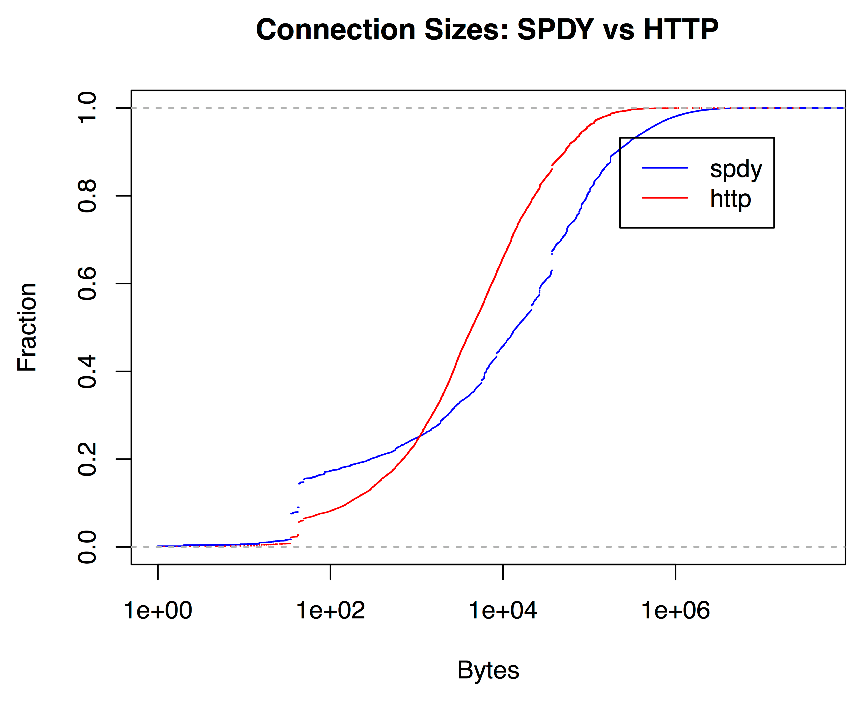
\includegraphics[width=0.4\textwidth]{plots/asset_combination_connection_sizes.eps}
\caption{Connection Sizes After Asset Combination}
\label{fig:connection-sizes}
\end{figure}

Figure \ref{fig:connection-sizes} describes the size of connections when all
assets are combined together as described in the SSL-and-IP combination
strategy. 70\% of SPDY connections are noticeably larger than HTTP connections,
up to almost an order of magnitude in some cases. Some assets do not benefit
from SPDY's combination: small assets like Google Analytics tracking
Javascript, or external libraries used on web pages such as jQuery. These
comprise the left part of the SPDY curve.

% we measure two approaches: splitting on SSL cert and IP and simply splitting
% on SSL cert (as an upper bound for combination). The first method, ssl + ip,
% is prone to some error due to the use of CDNs confusing our scraping of
% assets.

%%%%%%%%%%%%%%%%%%%%%%%%%%%%%%%%%%%%%%%%%%%%%%%%%%%%%%%%%%%%%%%%%%%%%%%%%%%%%%%
\section{Real World SPDY vs. HTTP}
\label{sec:realworld}
%%%%%%%%%%%%%%%%%%%%%%%%%%%%%%%%%%%%%%%%%%%%%%%%%%%%%%%%%%%%%%%%%%%%%%%%%%%%%%%
here is where we will discuss brian's spdyathome results


% I don't want to remove this wholesale but I don't think it is relevant
% anywhere else in the paper. Maybe it fits somewhere?
% -Tom
% %%%%%%%%%%%%%%%%%%%%%%%%%%%%%%%%%%%%%%%%%%%%%%%%%%%%%%%%%%%%%%%
% \section{Evaluation}
% \label{sec:eval}
% %%%%%%%%%%%%%%%%%%%%%%%%%%%%%%%%%%%%%%%%%%%%%%%%%%%%%%%%%%%%%%%
% Once this data is collected the time difference will be found between each
% protocol's retrieval of each test page. The obvious next step will be to
% determine if SPDY actually made the pages load faster or not. In all likelihood,
% there will not be a constant speedup across all pages and so the next step of
% evaluation will be to see in which cases an improvement was found. This should
% give insight into how SPDY improves over the prior specification and help decide
% whether or not it is worth it for the actual upgrade of HTTP to take place.
%
% This success of this experiment will be based off of how many points of data can
% be acquired and how varying the conditions are for them.  Much of what will be
% included in the final report will be plots and tables of the data collected to
% allow the reader to decide for themselves.  This information will be useful to
% others and the measurement platform itself should be designed in such a way that
% future experiments can be run on it without too much effort to retool it.

\bibliographystyle{plain}
\bibliography{rfc,citations}

\end{document}
